\begin{table}[htb!]
\begin{center}
\setlength{\tabcolsep}{0.0pc}
\caption{The number of observed data events and expected background contributions in the signal regions. 
The $p$-value of the observed events for the background-only hypothesis is denoted by $p(s = 0)$. 
The ``Rare'' category contains the contributions from associated production of $\ttbar$ with $h/WW/t/\ttbar$, 
as well as $tZ$, $Wh$, $Zh$, and triboson production. 
Background categories shown as ``$-$'' denote that they cannot contribute to a given region (charge flips or $W^\pm W^\pm jj$ in 3-lepton regions). 
The individual uncertainties can be correlated and therefore do not necessarily add up in quadrature to the total systematic uncertainty. 
}
\label{tab:SR_yields}
{\small
\begin{tabular*}{\textwidth}{@{\extracolsep{\fill}}lcccc}
\noalign{\smallskip}\hline\hline\noalign{\smallskip}
         & SR0b3j         & SR0b5j     & SR1b & SR3b     \\[-0.05cm]
\noalign{\smallskip}\hline\hline\noalign{\smallskip}
Observed events         & $3$     &  $3$  & $7$  & $1$            \\
\noalign{\smallskip}\hline\noalign{\smallskip}
Total background events & $1.5 \pm 0.4$ & $0.88 \pm 0.29$ & $4.5 \pm 1.0$ & $0.80 \pm 0.25$\\
$p(s = 0)$                &  0.13  &  0.04  &  0.15  &   0.36   \\
\noalign{\smallskip}\hline\noalign{\smallskip}
Fake/non-prompt leptons & $<0.2$ & $0.05\pm 0.18$ & $0.8 \pm 0.8$ & $0.13 \pm 0.17$\\
Charge-flip & $-$ & $0.02 \pm 0.01$ & $0.60 \pm 0.12$ & $0.19 \pm 0.06$\\
$t\bar{t}W$ & $0.02 \pm 0.01$ & $0.08 \pm 0.04$ & $1.1 \pm 0.4$ & $0.10 \pm 0.05$\\
$t\bar{t}Z$ & $0.10 \pm 0.04$ & $0.05 \pm 0.03$ & $0.92 \pm 0.31$ & $0.14 \pm 0.06$\\
$WZ$ & $1.2 \pm 0.4$ & $0.48 \pm 0.20$ & $0.18 \pm 0.11$ & $<0.02$\\
$W^\pm W^\pm jj$ & $-$ & $0.12 \pm 0.07$ & $0.03 \pm 0.02$ & $<0.01$\\
$ZZ$ & $<0.03$ & $<0.04$ & $<0.03$ & $<0.03$\\
Rare & $0.14 \pm 0.08$ & $0.07 \pm 0.05$ & $0.8 \pm 0.4$ & $0.24 \pm 0.14$\\  
\noalign{\smallskip}\hline\hline\noalign{\smallskip}
\end{tabular*}
}
\end{center}
\end{table}

\begin{figure}[t!]
\centering
\begin{subfigure}[t]{0.49\textwidth}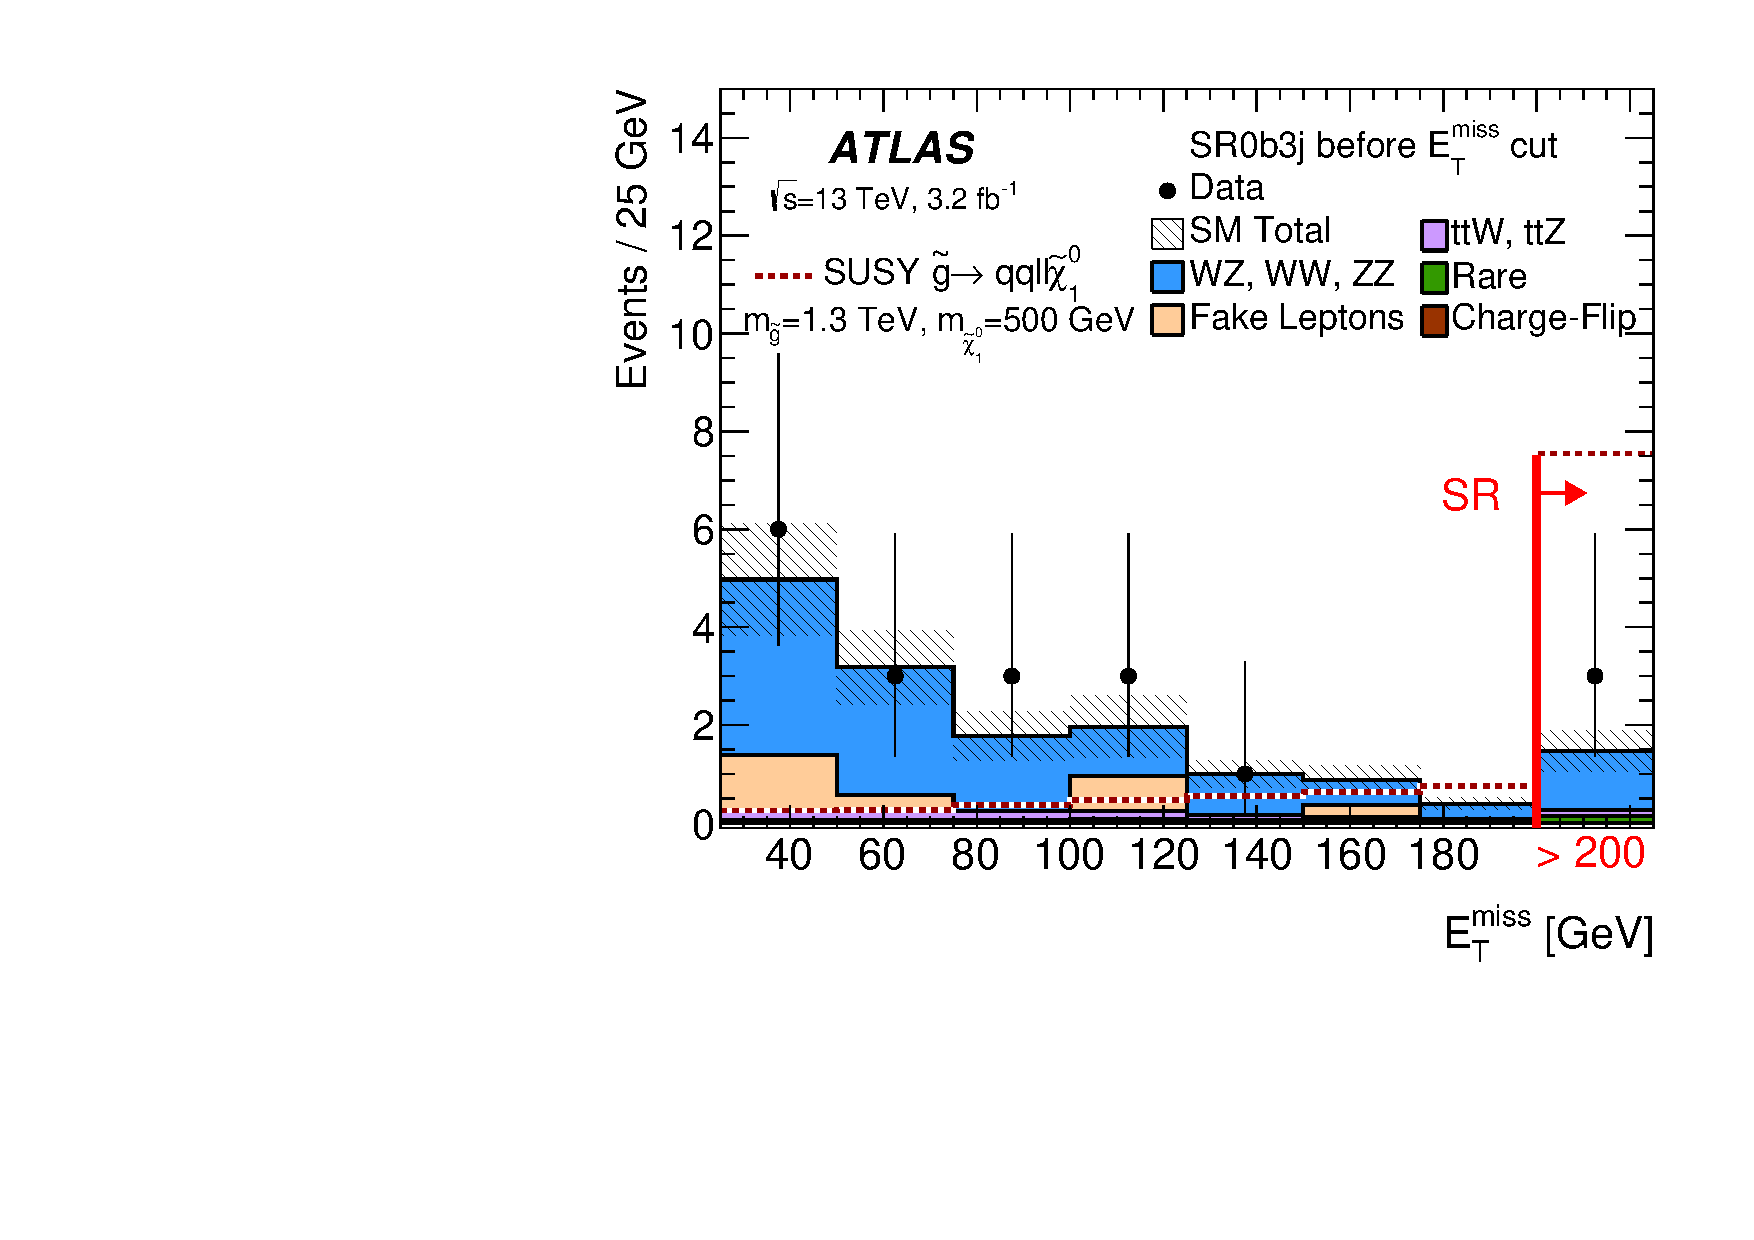
\includegraphics[width=\textwidth]{FIGURES/CONF_SR0b3j.pdf}
\caption{}\label{fig:Results_SR0b3j}\end{subfigure}
\begin{subfigure}[t]{0.49\textwidth}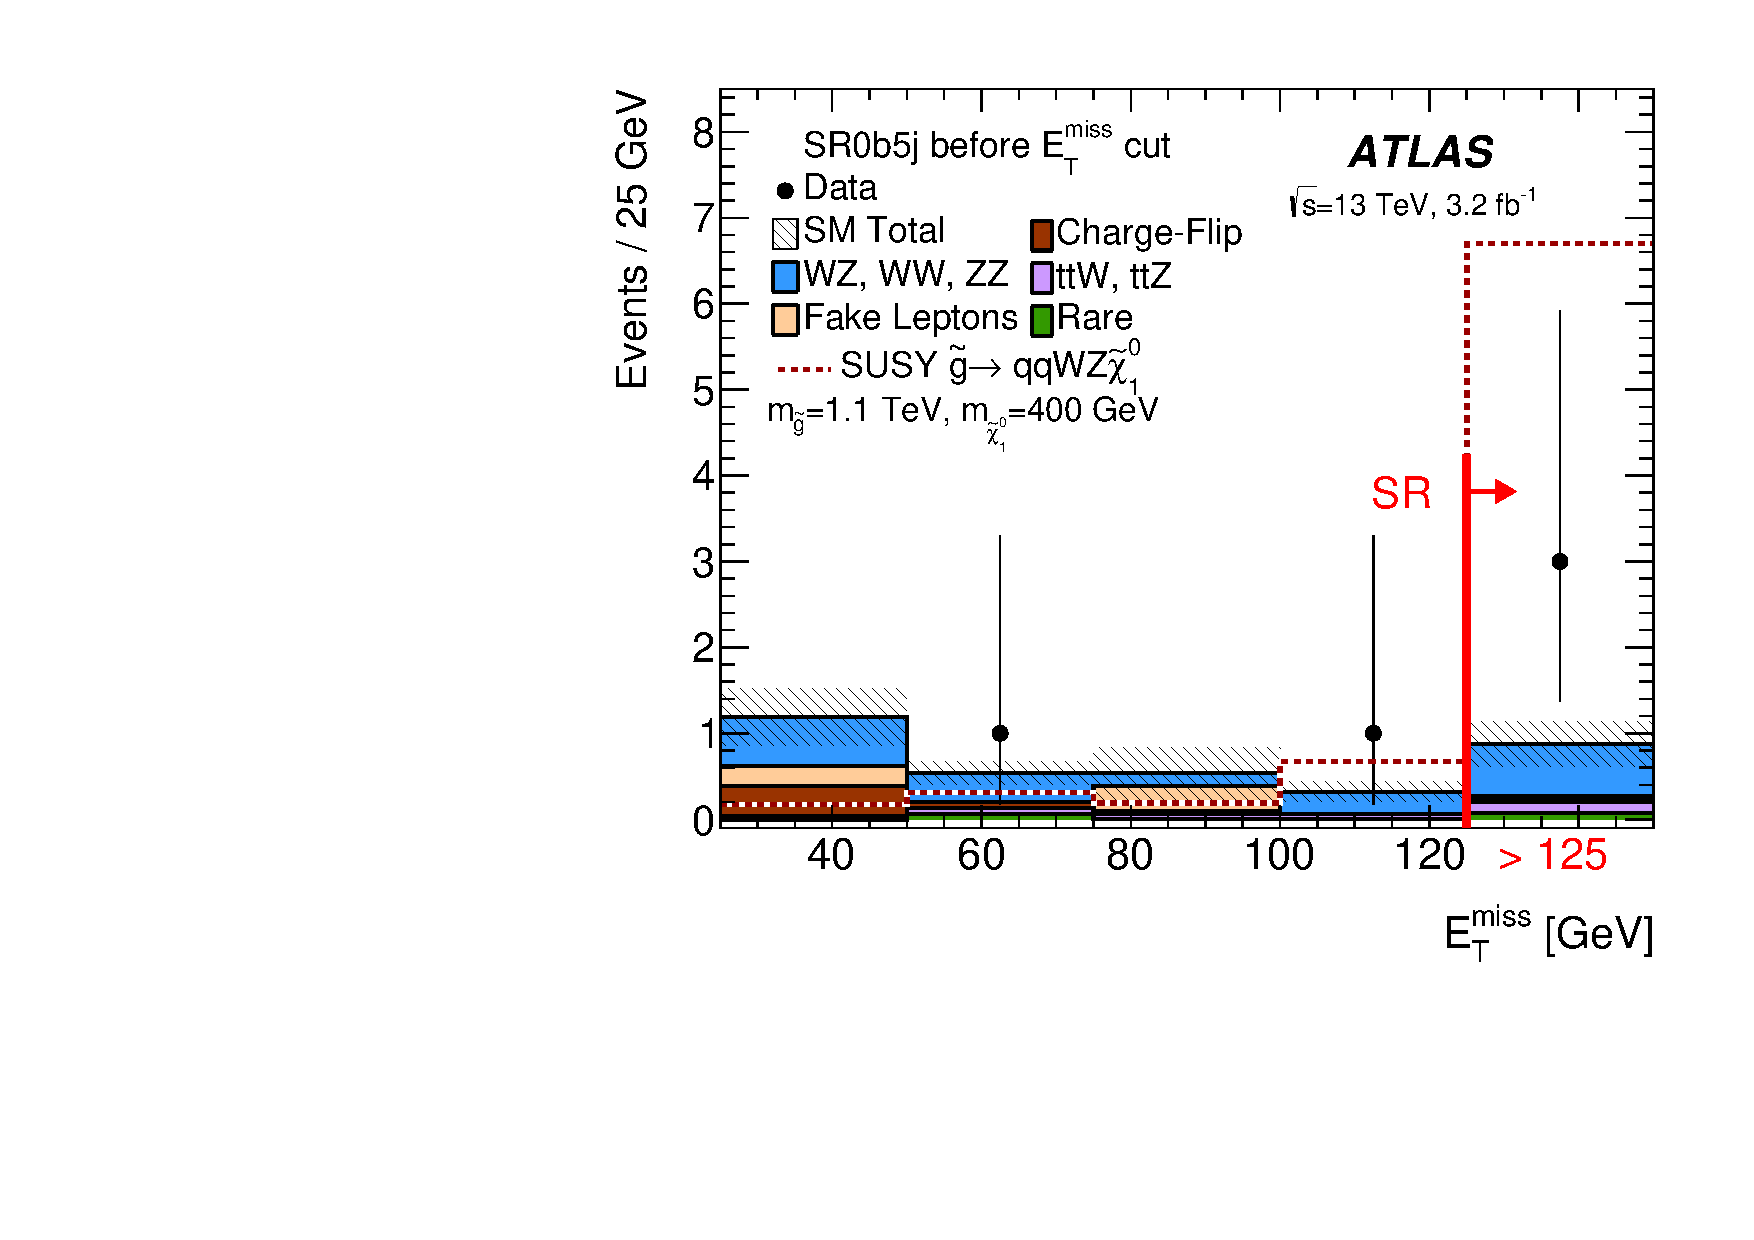
\includegraphics[width=\textwidth]{FIGURES/CONF_SR0b5j.pdf}
\caption{}\label{fig:Results_SR0b5j}\end{subfigure}
\begin{subfigure}[t]{0.49\textwidth}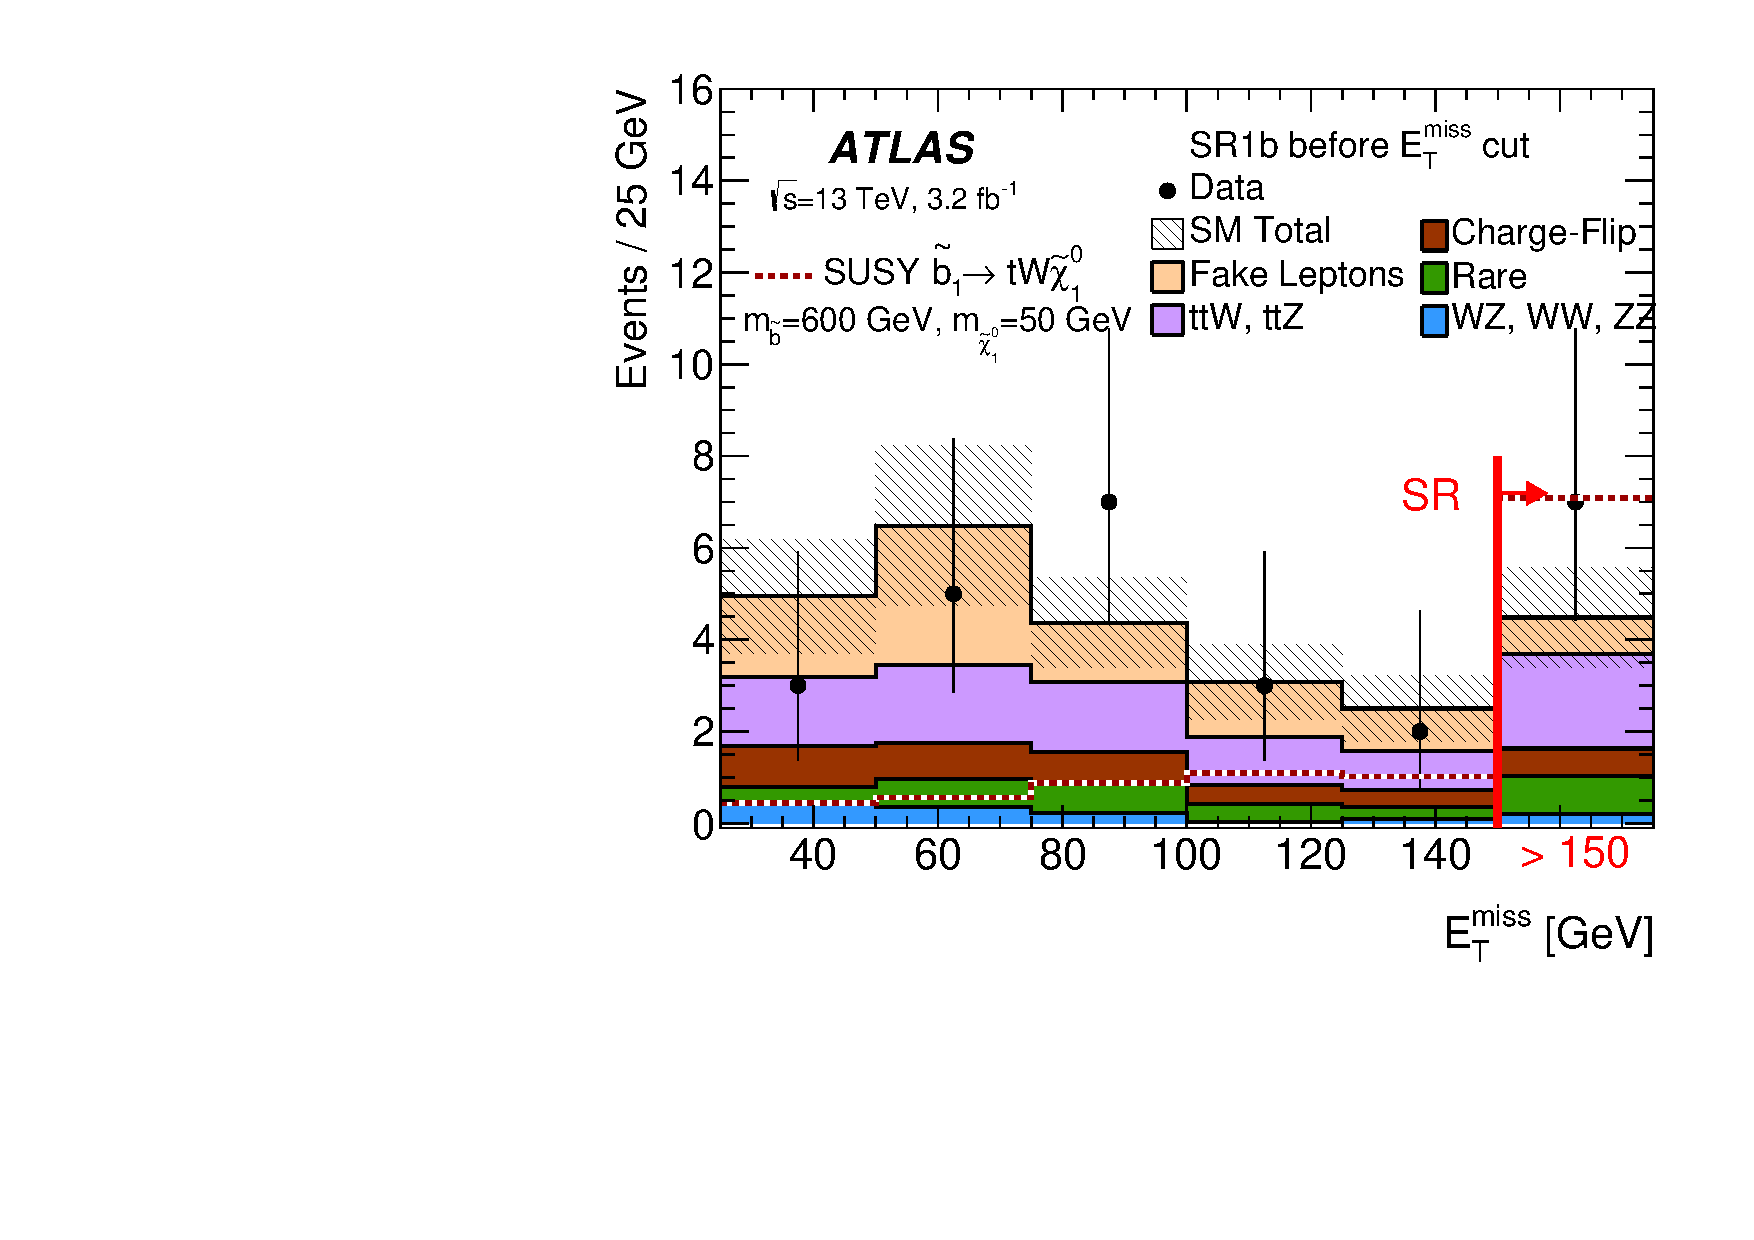
\includegraphics[width=\textwidth]{FIGURES/CONF_SR1b.pdf}
\caption{}\label{fig:Results_SR1b}\end{subfigure}
\begin{subfigure}[t]{0.49\textwidth}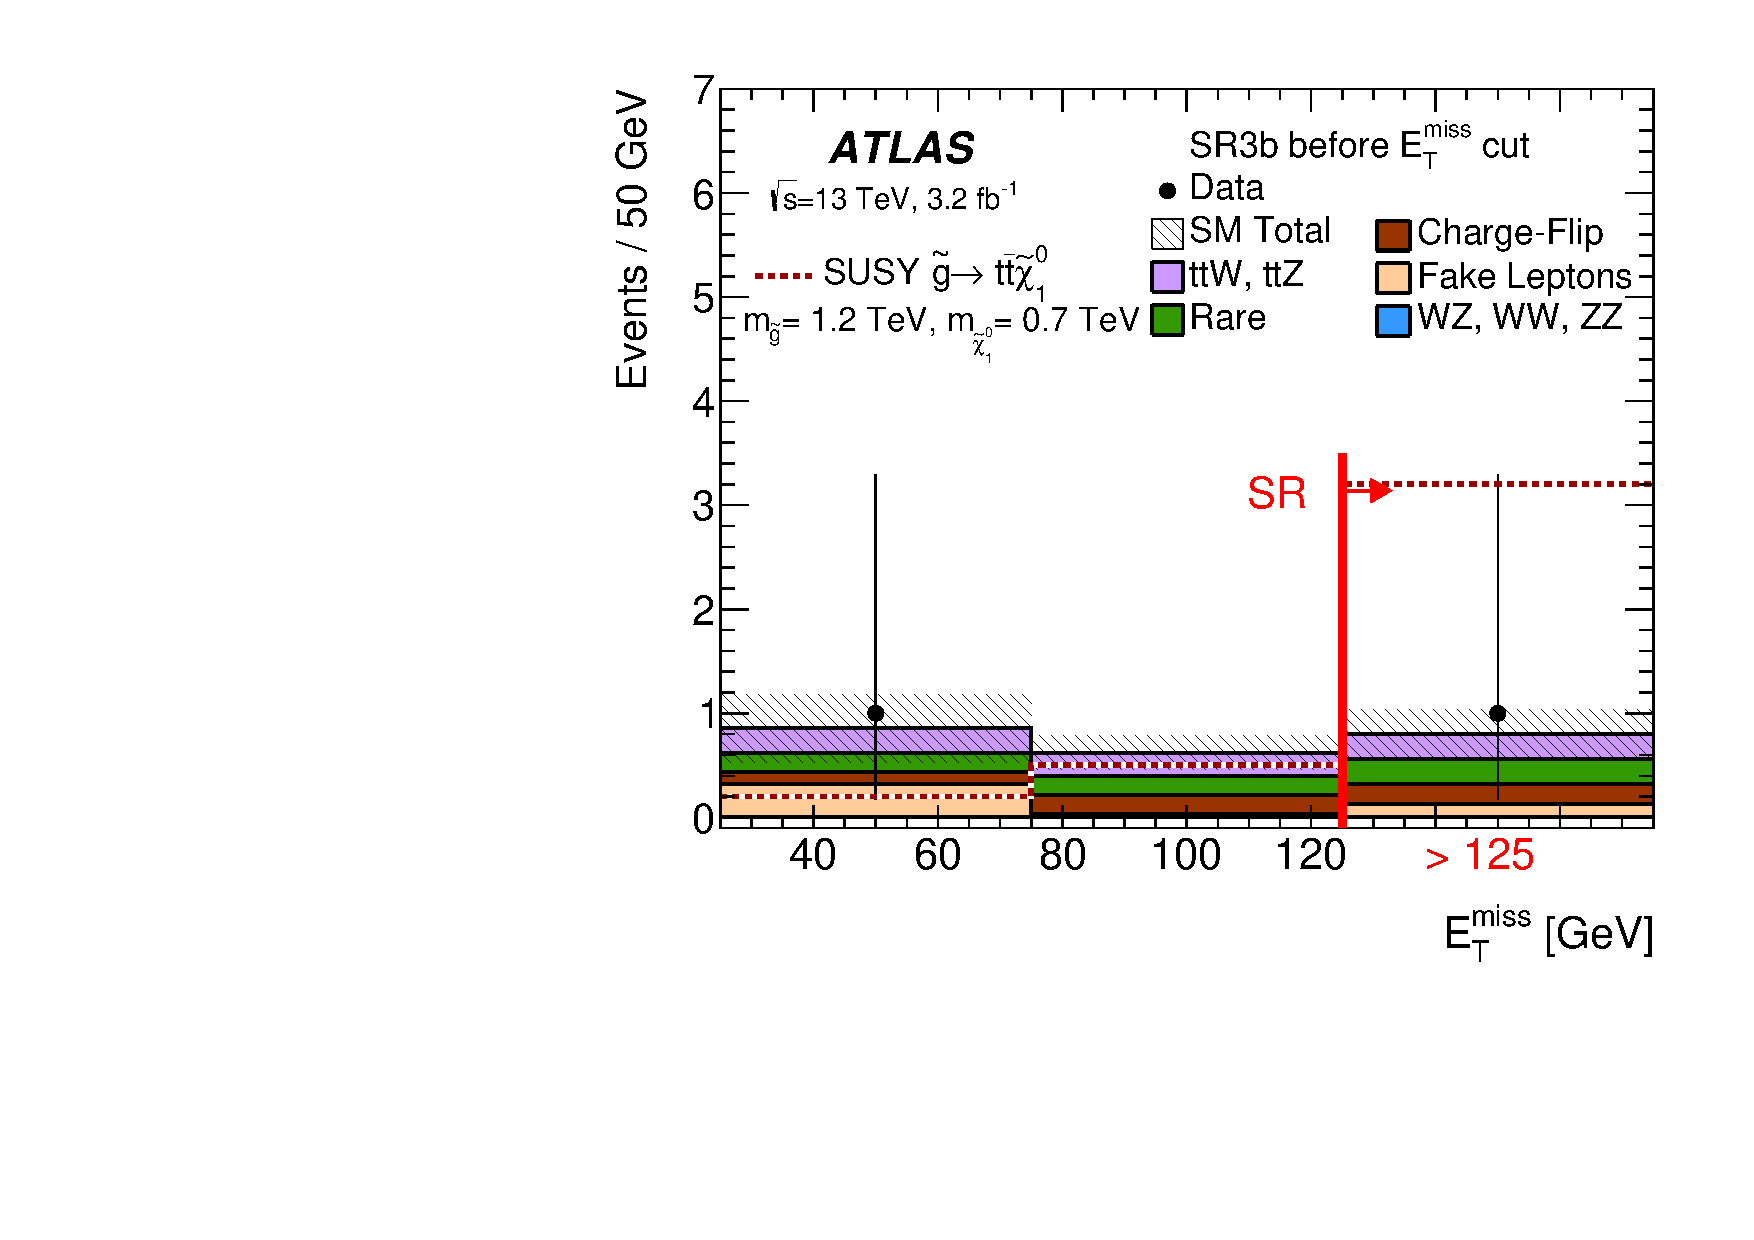
\includegraphics[width=\textwidth]{FIGURES/CONF_SR3b.pdf}
\caption{}\label{fig:Results_SR3b}\end{subfigure}
\caption{Missing transverse momentum distributions after (a) SR0b3j, (b) SR0b5j, (c) SR1b and (d) SR3b selection, beside the \met requirement. 
The results in the signal regions are shown in the last (inclusive) bin of each plot. 
The statistical uncertainties in the background prediction are included in the uncertainty band, 
as well as the theory uncertainties for the backgrounds with prompt SS/3L, 
and the full systematic uncertainties for data-driven backgrounds. 
The ``Fake leptons'' category corresponds to FNP leptons (see text), 
and the ``Rare'' category contains the contributions from associated production of $\ttbar$ with $h/WW/t/\ttbar$, 
as well as $tZ$, $Wh$, $Zh$, and triboson production. 
}
\label{fig:Results_SR_metD} 
\end{figure} 


Figure~\ref{fig:Results_SR_metD} shows the data \met distributions after the signal region selections (beside that on \met) in data 
together with the expected contributions from all the SM backgrounds with their total statistical and systematic uncertainties. 
For illustration, a typical SUSY signal distribution corresponding to the most relevant benchmark scenario 
in each SR is displayed.
The detailed yields for data and the different sources of SM background in the signal regions 
are presented in Table~\ref{tab:SR_yields}. 
The uncertainties amount to 22--34\% of the total background depending on the signal region. 
In all four SRs the number of data events exceeds the expectation but is consistent within the uncertainties, 
the smallest $p$-value for the SM-only hypothesis being 0.04 for SR0b5j. 
Out of the 14 events in the SRs, 2 of the events in SR1b and the 3 events in SR0b3j contain three leptons. 
None of those events contain three leptons of equal charge. 

In the absence of any significant deviations from the SM predictions, upper limits on possible BSM contributions to the signal regions are computed, 
in particular in the context of the SUSY benchmark scenarios described in Section~\ref{sec:intro}. 
The HistFitter framework~\cite{Baak:2014wma}, which utilises a profile-likelihood-ratio test~\cite{Cowan:2010js}, 
is used to establish 95\% confidence intervals using the CL$_\mathrm{s}$ prescription~\cite{Read_CLs}. 
The likelihood is built as the product of a Poisson probability density function describing the observed number of events in the signal region 
and Gaussian distributions constraining the nuisance parameters 
associated with the systematic uncertainties whose widths correspond to the sizes of these uncertainties; 
Poisson distributions are used instead for MC statistical uncertainties. 
Correlations of a given nuisance parameter across the different sources of backgrounds and the signal are taken into account when relevant. 
The statistical tests are performed independently for each of the signal regions. 

Table~\ref{tab:upperlimits} presents 95\% confidence level (CL) model-independent upper limits 
on the number of BSM events, $N_\mathrm{BSM}$, that may contribute to the signal regions. 
Normalising these by the integrated luminosity $L$ of the data sample, they can be interpreted as upper limits on the visible BSM cross-section $\sigma_{\rm{vis}}$, 
defined as the product $\sigma_{\rm{prod}}\times A \times\epsilon=N_\mathrm{BSM}/L$ of production cross-section, acceptance and reconstruction efficiency. 

\begin{table}[htb!]
\centering
\caption{Signal model-independent upper limits on the number of BSM events ($N_{\rm{BSM}}$) 
  and the visible signal cross-section ($\sigma_{\rm{vis}}$) in the four SRs. 
  The numbers (in parentheses) give the observed (expected under the SM hypothesis) 95\% CL upper
  limits. Calculations are performed with pseudo-experiments.
  The $\pm$1$\sigma$ variations on the expected limit due to the statistical and systematic uncertainties in the background prediction are also shown. 
}
\label{tab:upperlimits}
{\small
\renewcommand{\arraystretch}{1.4}
\begin{tabular*}{\textwidth}{@{\extracolsep{\fill}}lrrrr}
\noalign{\smallskip}\hline\hline\noalign{\smallskip}
         & SR0b3j         & SR0b5j     & SR1b & SR3b     \\[-0.05cm]
\noalign{\smallskip}\hline\hline\noalign{\smallskip}
$N_{\rm{BSM}}^{\rm{obs}}$ ($N_{\rm{BSM}}^{\rm{exp}}$) 
 & $5.9$  $({4.1}^{+1.6}_{-0.8})$
 & $6.4$ $({3.6}^{+1.2}_{-1.1})$
 & $8.8$ $({6.0}^{+2.6}_{-1.6})$ 
 & $3.8$ $({3.7}^{+1.1}_{-0.5})$ \\
$\sigma_{\rm{vis}}^{\rm{obs}}$ [fb] & 1.8 & 2.0 & 2.8 & 1.2\\
\noalign{\smallskip}\hline\hline\noalign{\smallskip}
  \end{tabular*}
}
\end{table} 

\begin{figure}[htb!]
\centering
\begin{subfigure}[t]{0.49\textwidth}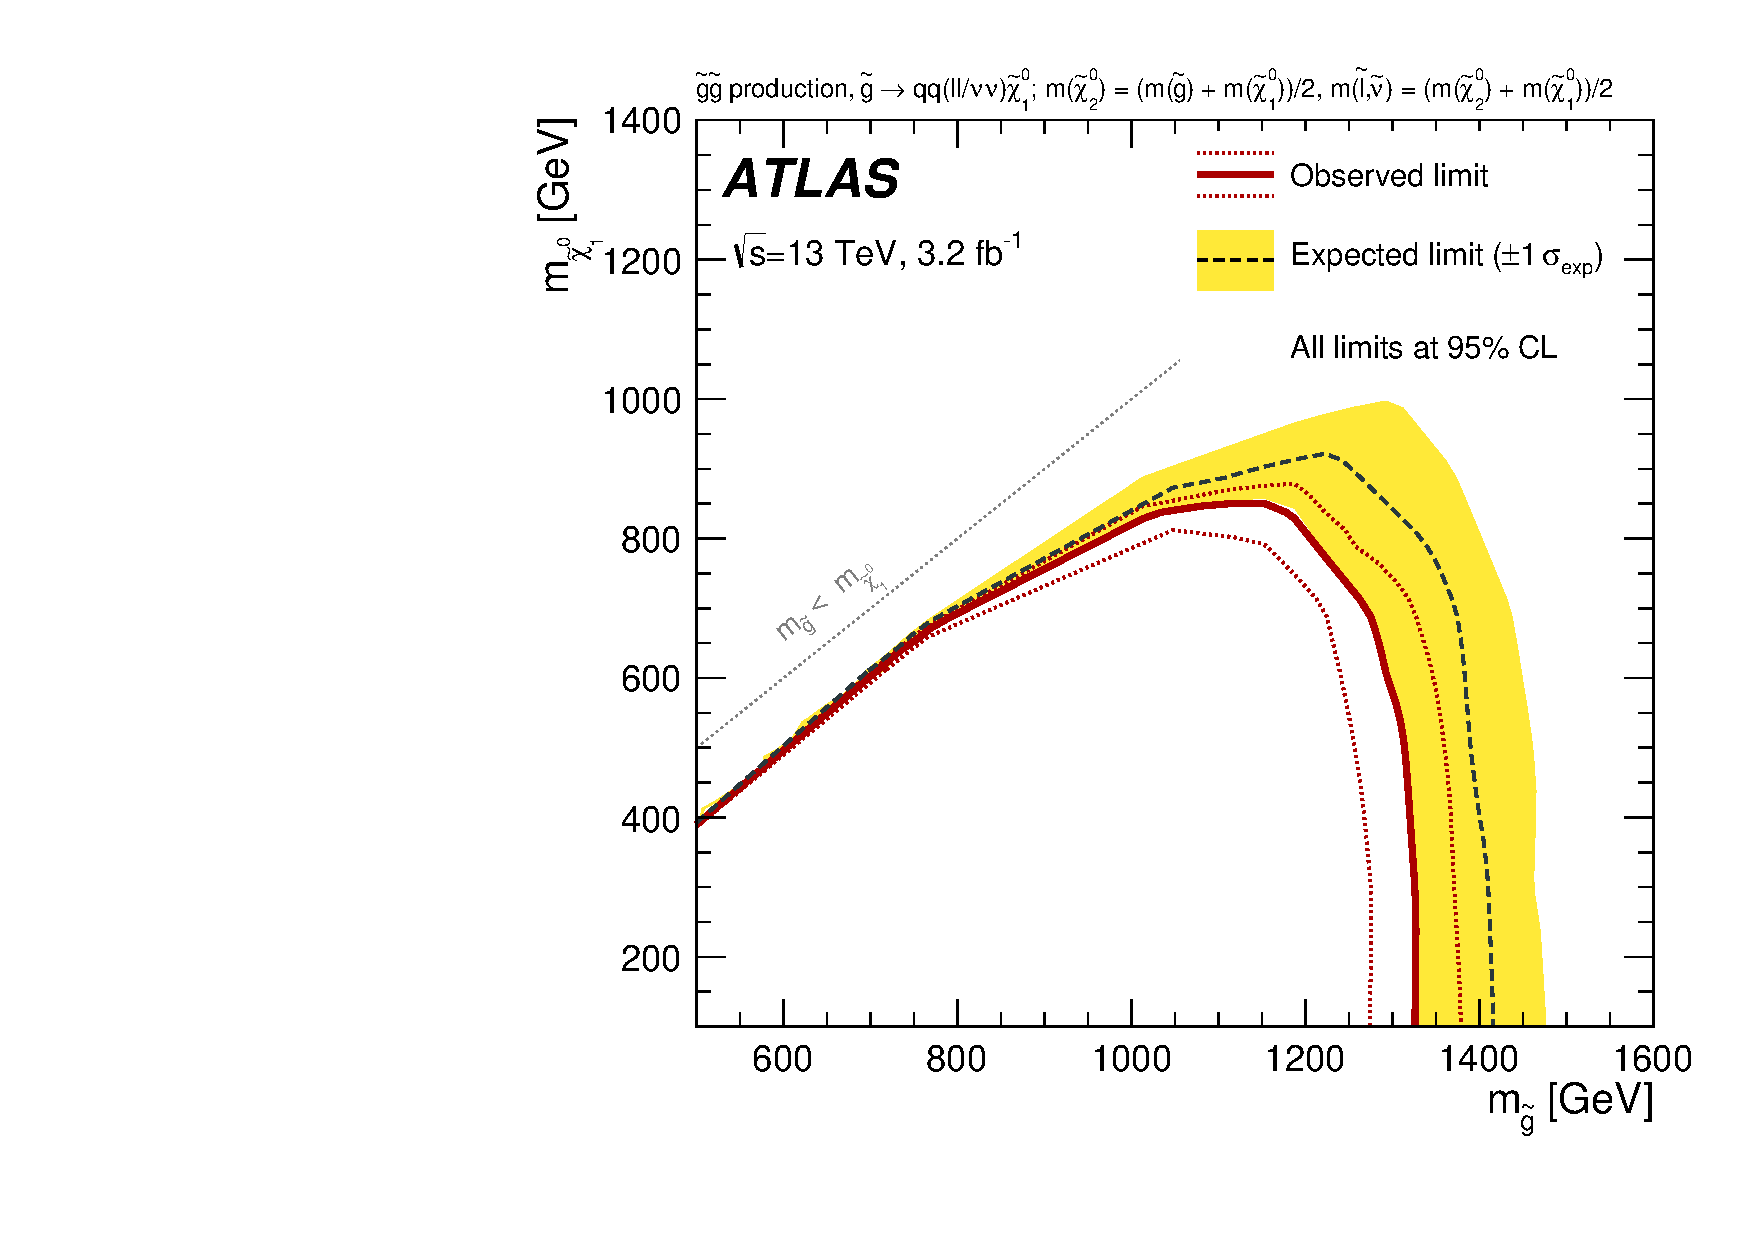
\includegraphics[width=\textwidth]{exclusion2015SameSign_SR0b3j.pdf}
\caption{$\gluino\to q\bar q \ell\ell\ninoone$ scenario, SR0b3j}\label{fig:limits_SR0b3j}\end{subfigure}
\begin{subfigure}[t]{0.49\textwidth}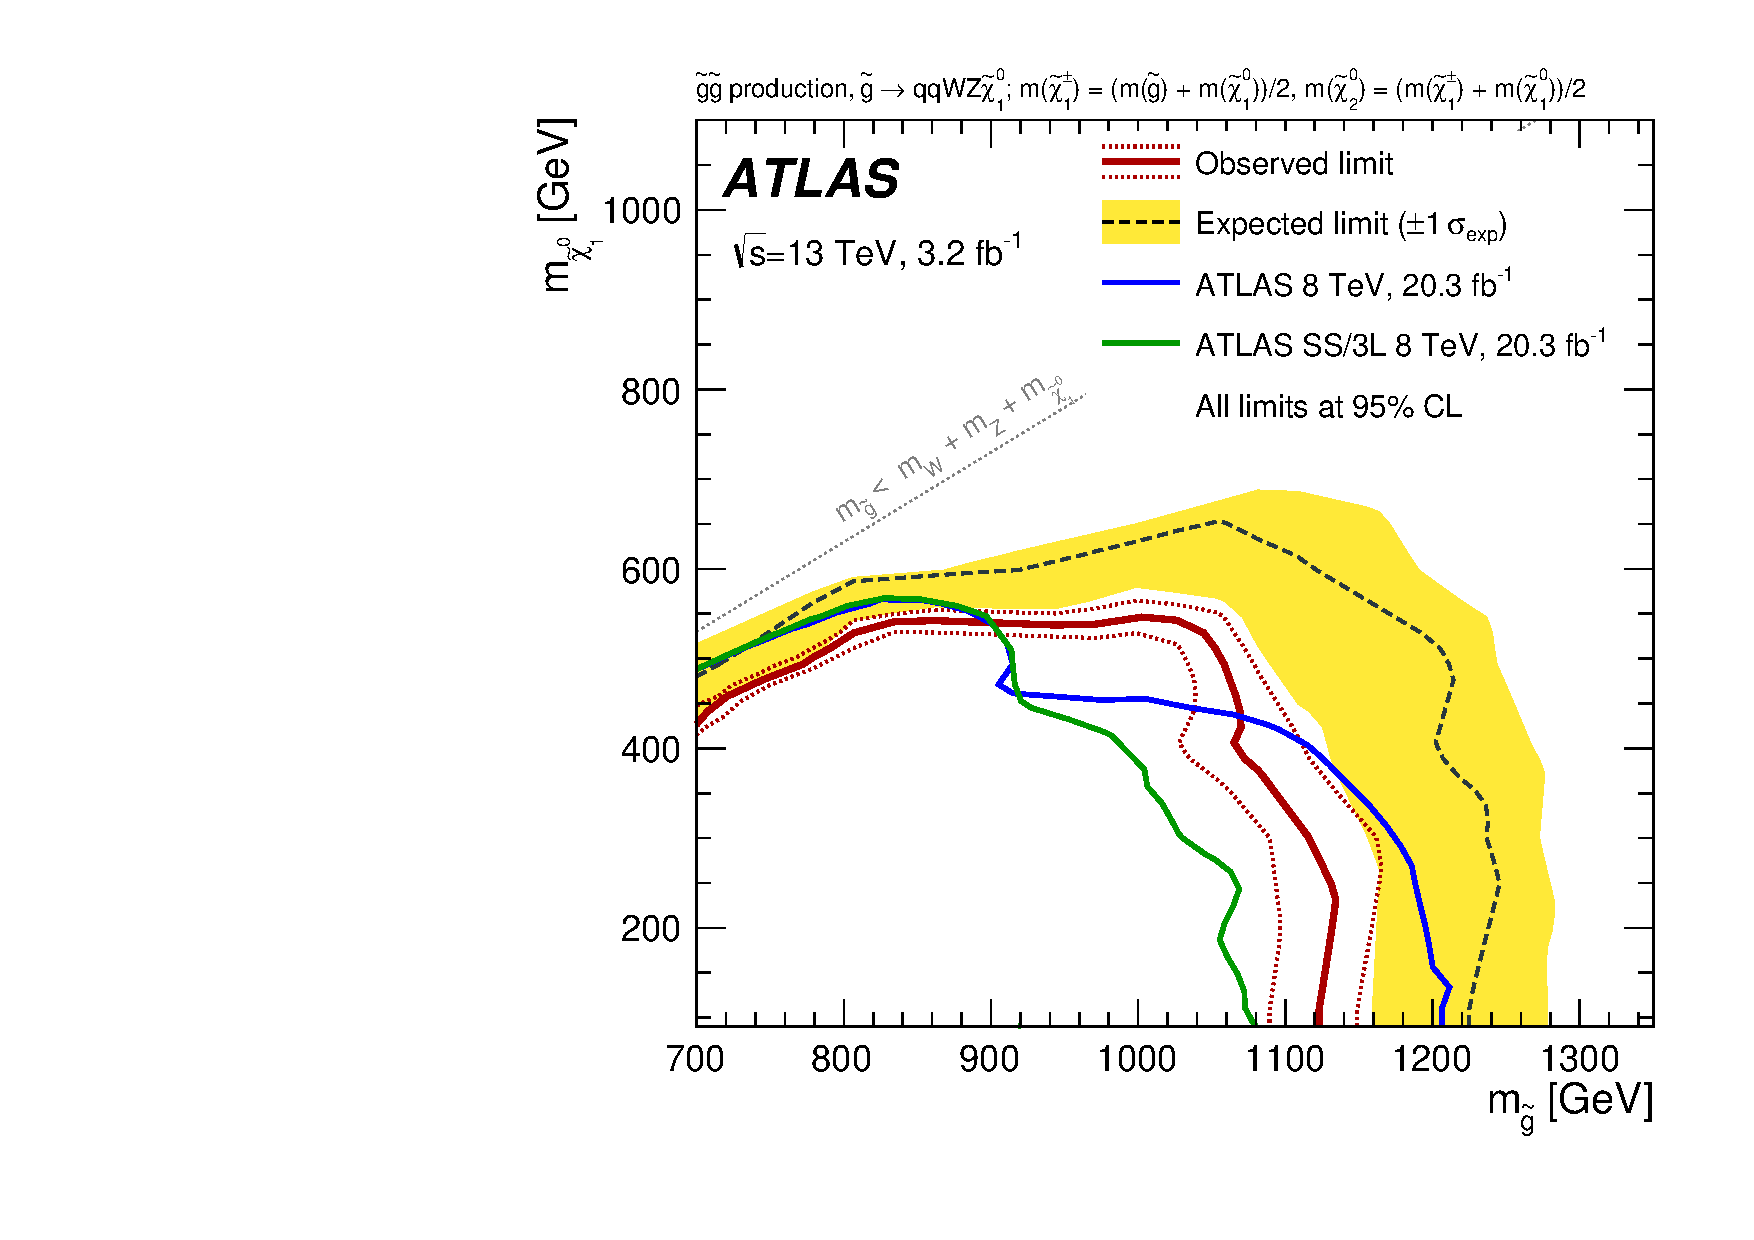
\includegraphics[width=\textwidth]{exclusion2015SameSign_SR0b5j.pdf}
\caption{$\gluino\to q\bar q' WZ\ninoone$ scenario, SR0b5j}\label{fig:limits_SR0b5j}\end{subfigure}
\par\bigskip
\begin{subfigure}[t]{0.49\textwidth}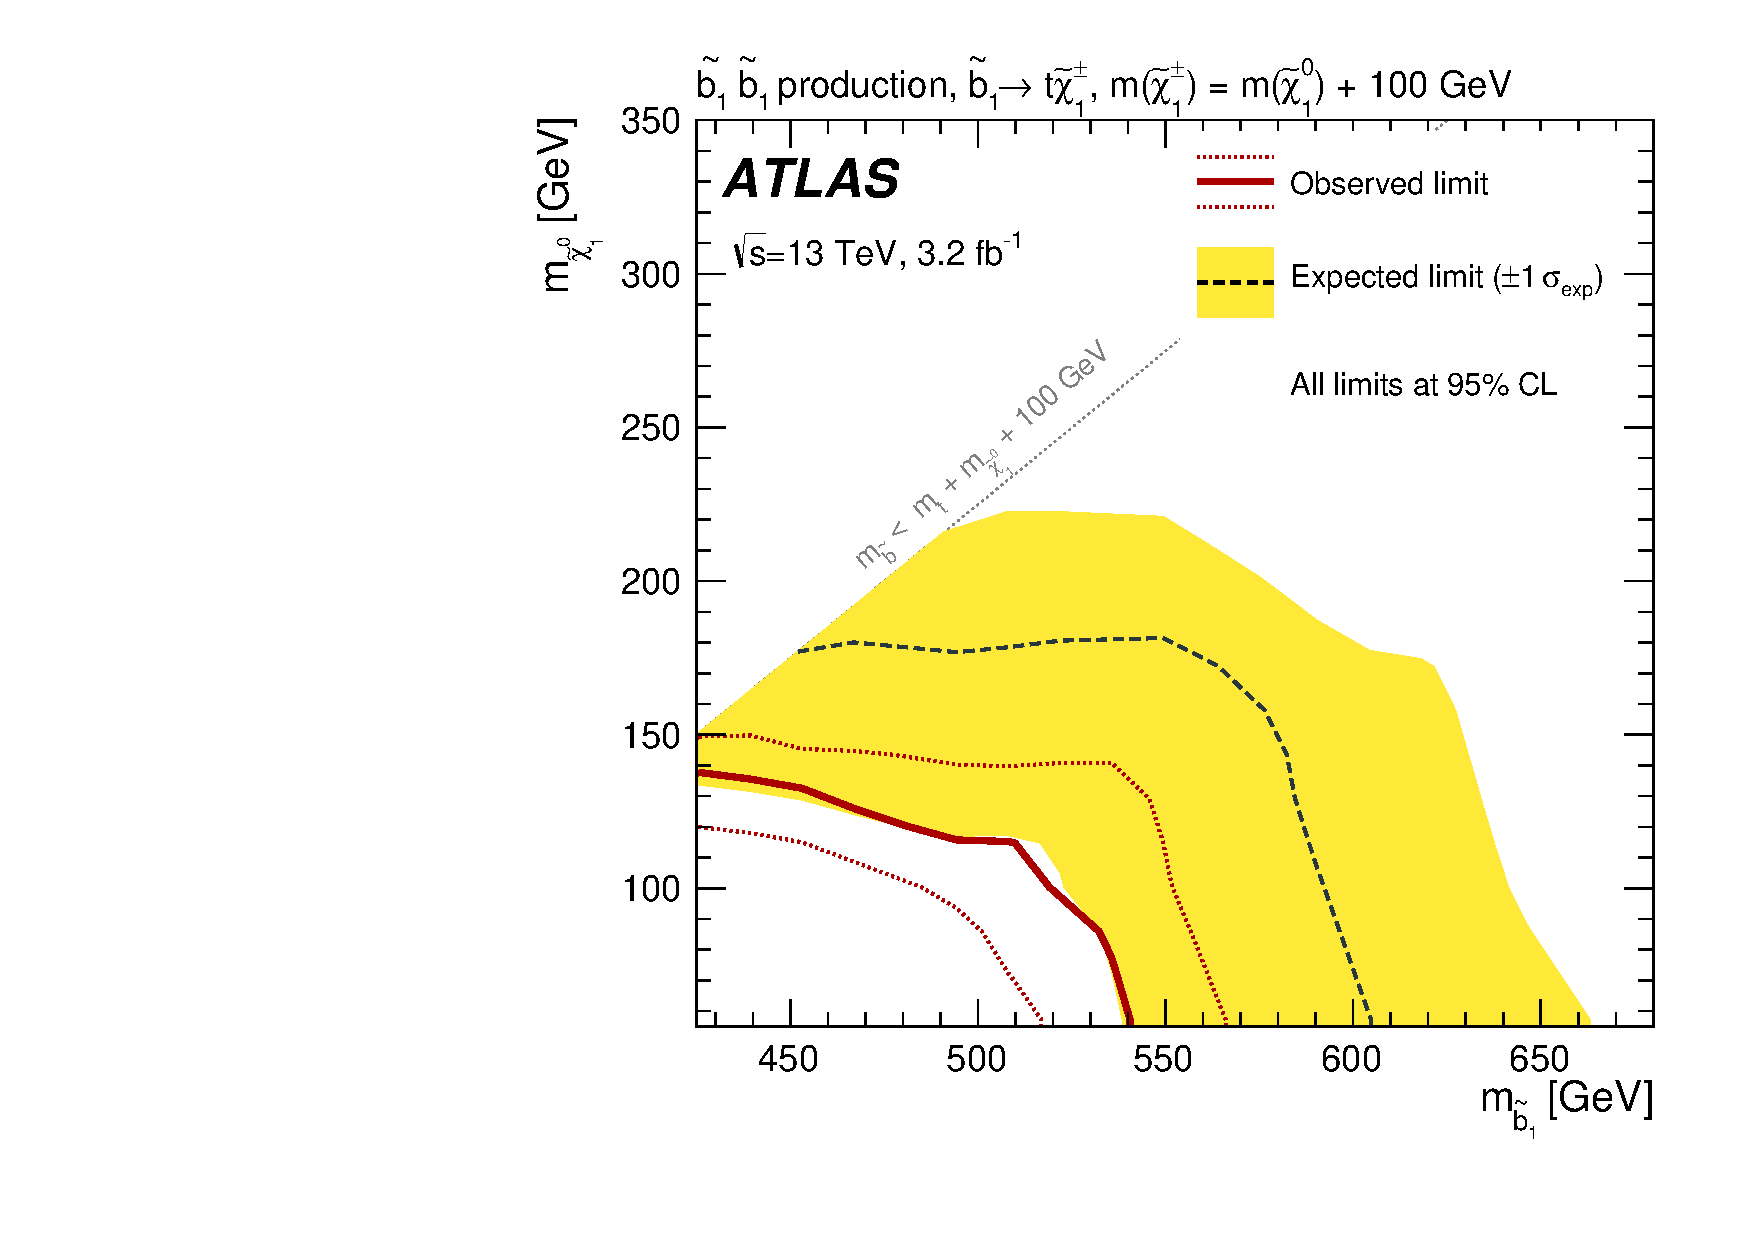
\includegraphics[width=\textwidth]{exclusion2015SameSign_SR1b.pdf}
\caption{$\sbottomone\to tW^-\ninoone$ scenario, SR1b}\label{fig:limits_SR1b}\end{subfigure}
\begin{subfigure}[t]{0.49\textwidth}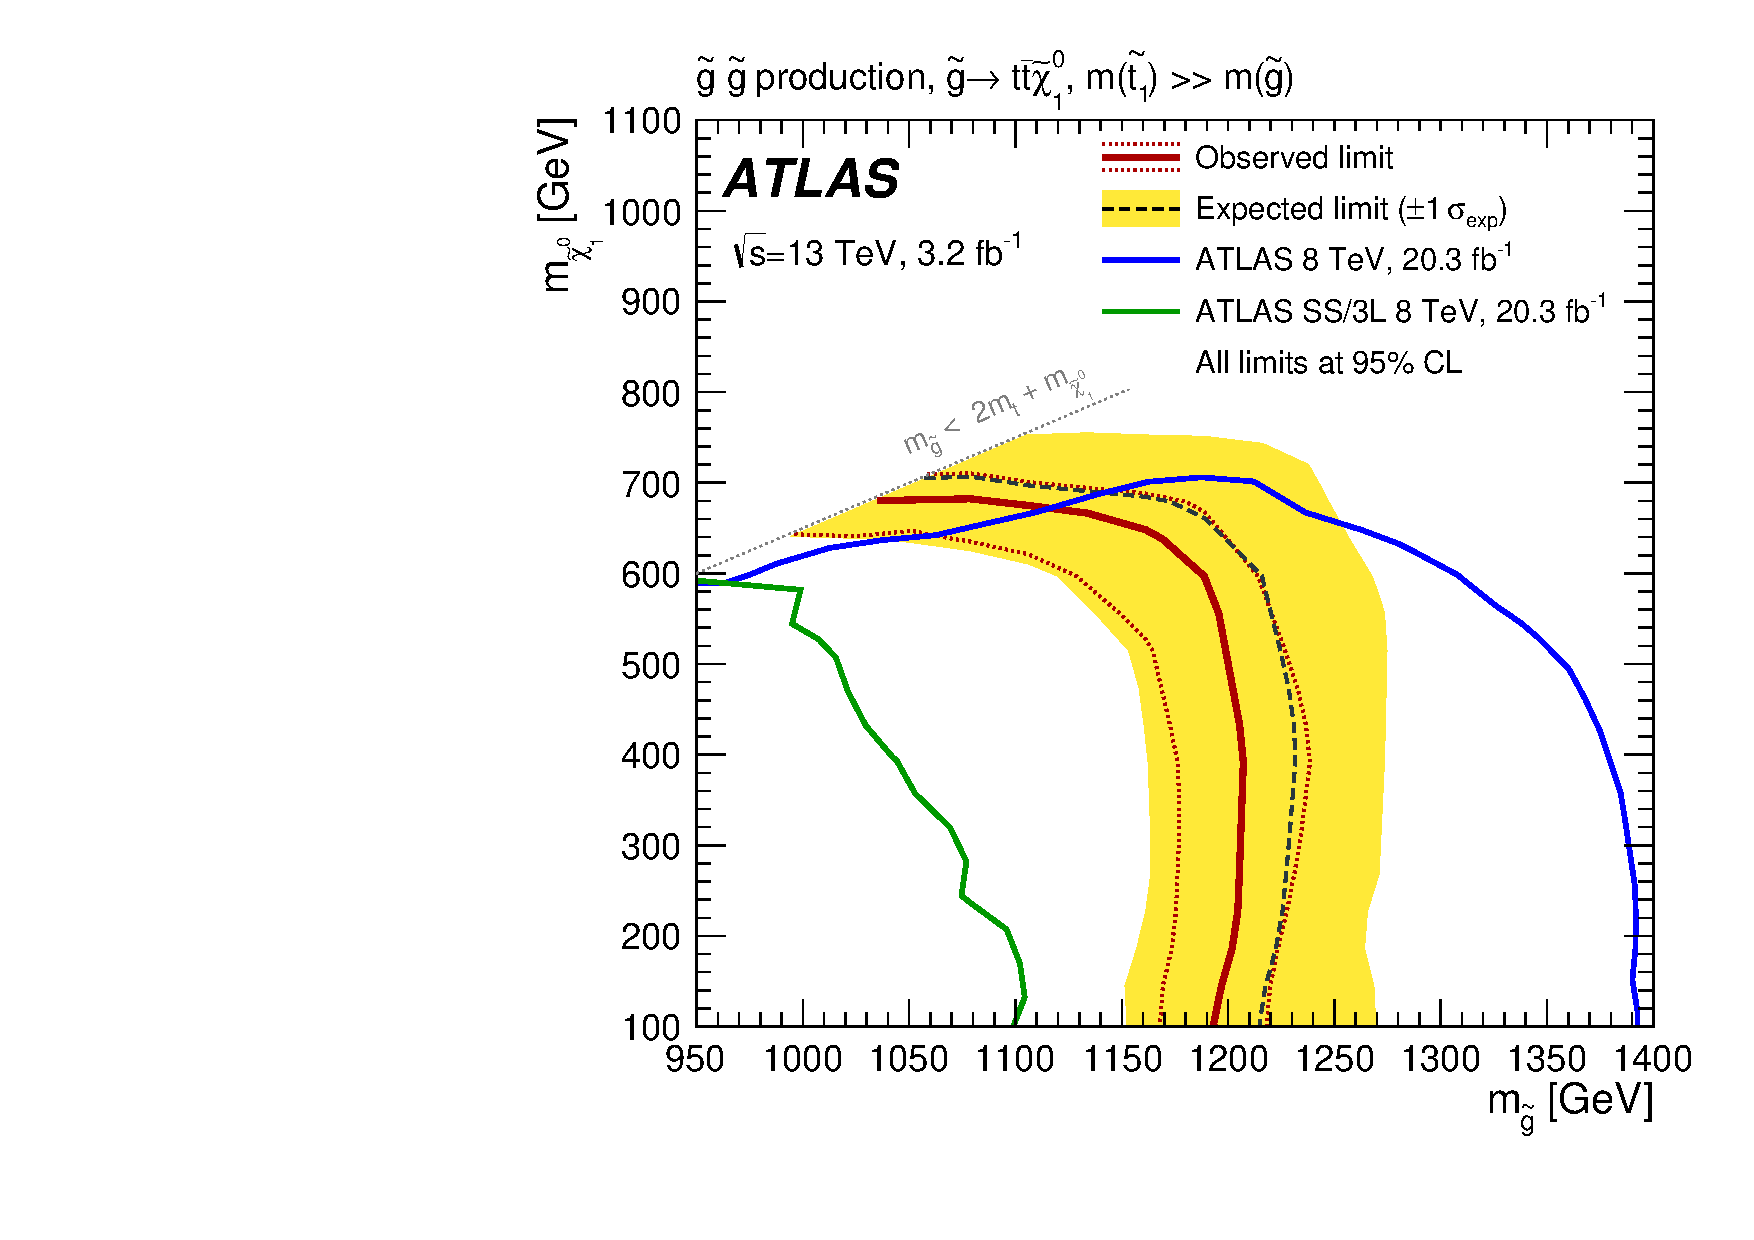
\includegraphics[width=\textwidth]{exclusion2015SameSign_SR3b.pdf}
\caption{$\gluino\to t\bar t\ninoone$ scenario, SR3b}\label{fig:limits_SR3b}\end{subfigure}
\caption{
Observed and expected exclusion limits on the \gluino, \sbottomone and \ninoone masses 
in the context of SUSY scenarios with simplified mass spectra 
featuring $\gluino\gluino$ or $\sbottomone\sbottomonebar$ pair production with exclusive decay modes. 
The signal region used to obtain the limits is specified for each scenario. 
The contours of the band around the expected limit are the $\pm$1$\sigma$ results, 
  including all uncertainties except theoretical uncertainties on the signal cross-section. The dotted lines around the observed
    limit illustrate the change in the observed limit as the nominal signal cross-section is scaled up and down
    by the theoretical uncertainty. All limits are computed at 95\% CL. 
    The diagonal lines indicate the kinematic limit for the decays in each specified scenario.  
For figures (b) and (d), results are compared with the observed limits obtained by previous ATLAS searches~\cite{paperSS3L,Aad:2015iea,Aad:2015pfx}. 
For figures (a) and (c), a direct comparison with earlier searches is not possible, due to differing model assumptions. 
}
\label{fig:Results_Limits} 
\end{figure} 

Exclusion limits are also set on the masses of the superpartners involved in the four SUSY benchmark scenarios considered in this analysis. 
Simplified models corresponding to a single production mode and with 100\% branching ratio to a specific decay chain are used, 
with the masses of the SUSY particles not involved in the process set to very high values. 
Figure~\ref{fig:Results_Limits} shows the limits 
on the mass of the $\ninoone$ as a function of the $\gluino$ or $\sbottomone$ mass. 
%For these results, asymptotic formulas~\cite{Cowan:2010js} are used to model the probability distribution of the test statistic. 
In some cases, the new limits set by this analysis can be compared 
with the existing limits set by the combination of ATLAS SUSY searches with 8 TeV data~\cite{Aad:2015iea,Aad:2015pfx}. 
For parts of the parameter space, the sensitivity reached with the 13 TeV dataset exceeds that of the 8 TeV dataset,
and additional parameter space regions can be excluded, especially for large neutralino masses. 

Signal models featuring gluino pair production with a subsequent gluino decay via $\ninotwo$ and light sleptons\\ 
($\gluino\to q\bar q\ninotwo\to q\bar q (\ell\slepton^*/\nu\tilde{\nu}^*)\to q\bar q(\ell^+\ell^-/\nu\nu)\ninoone$) 
are probed using SR0b3j (Fig.~\ref{fig:limits_SR0b3j}).
In this simplified model, the gluinos decay into $u\bar u$, $d\bar d$, $s\bar s$ or $c\bar c$ with equal probabilities, 
and the six types of leptons are also produced in the $\tilde\chi_2^0$ decays with equal probabilities. 
The $\ninotwo$ mass is set to $m_{\ninotwo}=(m_{\gluino} + m_{\ninoone})/2$, 
with the $\slepton$ and $\tilde{\nu}$ masses set to $m_{\slepton,\tilde{\nu}}=(m_{\ninotwo} + m_{\ninoone})/2$.
Gluino masses up to $m_{\gluino}\approx\SI{1.3}{TeV}$ for a light \ninoone and \ninoone masses up to $m_{\ninoone}\approx\SI{850}{GeV}$ for gluinos with $m_{\gluino}\approx\SI{1.1}{TeV}$ are excluded in this scenario. 

Similarly, models with gluino production  with a subsequent two-step gluino decay via $\chinoonepm$ and $\ninotwo$\\ 
($\gluino\to q\bar q \chinoonepm \to q\bar q W\ninotwo \to  q\bar q W Z \ninoone$) 
are probed with SR0b5j (Fig.~\ref{fig:limits_SR0b5j}).
In this simplified model, the gluinos decay into $u\bar u$, $d\bar d$, $s\bar s$ or $c\bar c$ with equal probabilities. 
The $\chinoonepm$ mass is set to $m_{\chinoonepm}=(m_{\gluino} + m_{\ninoone})/2$ and
the $\ninotwo$ mass is set to $m_{\ninotwo}=(m_{\chinoonepm} + m_{\ninoone})/2$; 
$W$ and $Z$ bosons produced in the decay chain are not necessarily on-shell. 
The exclusion limits in this scenario reach $m_{\gluino}\approx\SI{1.1}{TeV}$ (for light $\ninoone$) and $m_{\ninoone}\approx\SI{550}{GeV}$ (for $m_{\gluino}\approx\SI{1.0}{TeV}$).

Exclusion limits in a simplified model of bottom squark production with chargino-mediated $\sbottomone\to tW^-\ninoone$ decays are 
obtained with SR1b (Fig.~\ref{fig:limits_SR1b}).
In this model the $\chinoonepm$ mass is set to $m_{\chinoonepm}=m_{\ninoone} + \SI{100}{GeV}$.
The limits can reach mass values of $m_{\sbottomone}\approx\SI{540}{GeV}$ for a light $\ninoone$, 
while $m_{\ninoone}\lesssim\SI{140}{GeV}$ are also excluded for $m_{\sbottomone}\approx\SI{425}{GeV}$, 
significantly extending the previous limits obtained at $\sqrt{s}=8$~TeV~\cite{Aad:2015pfx} 
which excluded $m_{\sbottomone}\lesssim\SI{470}{GeV}$ for $m_{\ninoone}\approx\SI{60}{GeV}$ for a similar model.

Finally, SR3b is used to set limits on masses in a simplified model with 
gluino pair production and $\gluino\to t\bar t\ninoone$ decays 
via an off-shell top squark (Fig.~\ref{fig:limits_SR3b}). 
In that case, gluino masses of $m_{\gluino}\lesssim\SI{1.2}{TeV}$ are excluded for $m_{\ninoone}\lesssim\SI{600}{GeV}$, 
and $\ninoone$ masses up to $m_{\ninoone}\approx\SI{680}{GeV}$ are also excluded for $m_{\gluino}\approx\SI{1.05}{TeV}$. 
